\documentclass[fleqn]{article}

\usepackage{mydefs}
\usepackage{notes}
\usepackage{url}
\usepackage{graphicx}
\usepackage{textcomp}
\graphicspath{ {../output/} }

\begin{document}
\lecture{Computer Vision}{HW2: Feature Detection and Panoramas}{Dan Engbert, QD36731}

{\bf Section 1 - Coding Assignment} 
\\
The goal of this assignment is to implement robust homography estimation to stitch pairs of images together.

My strategy for completing this assignment:
\bee
\i Use cv2.goodFeaturesToTrack() to perform harris corner detection so as to identify feature points in each image.
\i Around each feature point I looked at the 20x20 neighborhood of grayscale pixels and stored their intensities in a 1D vector.
\i Points were then paired up between each image using the euclidean distance between each vector.
\i Some (ambiguous) pairs were removed if a feature point vector in one image matched too closely with two feature points in the other image (their distances were within 75\% of each other).
\i Then RANSAC was performed by selecting random sets of 4 pairs, computing the perspective transformation needed, and then testing the transformation on the rest of the pairs.  Pairs were considered inliners if the predicted pixel location was within 8 pixels of the location from the pair. After 10,000 iterations, the model with the most inliners was taken as the final model to use.
\i The model was then applied to one image with cv2.warpPerspective() and then translated and combined with the second image (averaging pixels where they overlap).
\i For panoramas created with 3 images, the above steps were completed using two of the images, and then completed again using the result and the third image.
\ene


{\bf Section 2.1 - Tower Images:} 

The image below shows all the feature points detected for the tower images (after removing ambigous pairs (step 4 in section 1 above).  Pairs are shown as randomly colored squares, with the corresponding points in each image having the same color:
\begin{center}
  \makebox[\textwidth]{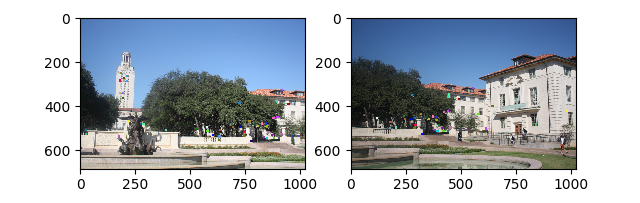
\includegraphics[width=0.7\paperwidth]{features-tower.png}}
\end{center}

The image below shows all the inliner points for the final model from ransac() on the tower image:
\begin{center}
  \makebox[\textwidth]{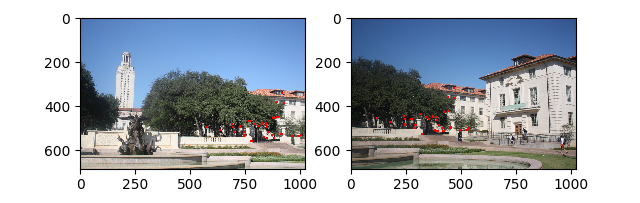
\includegraphics[width=0.7\paperwidth]{inliners-tower.png}}
\end{center}

The final model had 29 inliners (out of 55 pairs in total) and the average residual for the inliners was 0.726495018323.

Final model matrix:

[[  1.30249313e+00  -5.69817380e-02  -5.83153966e+02]

 [  1.66460590e-01   1.23334766e+00  -1.69296782e+02]

 [  2.71519447e-04   4.69769503e-05   1.00000000e+00]]

Output Panorama:
\begin{center}
  \makebox[\textwidth]{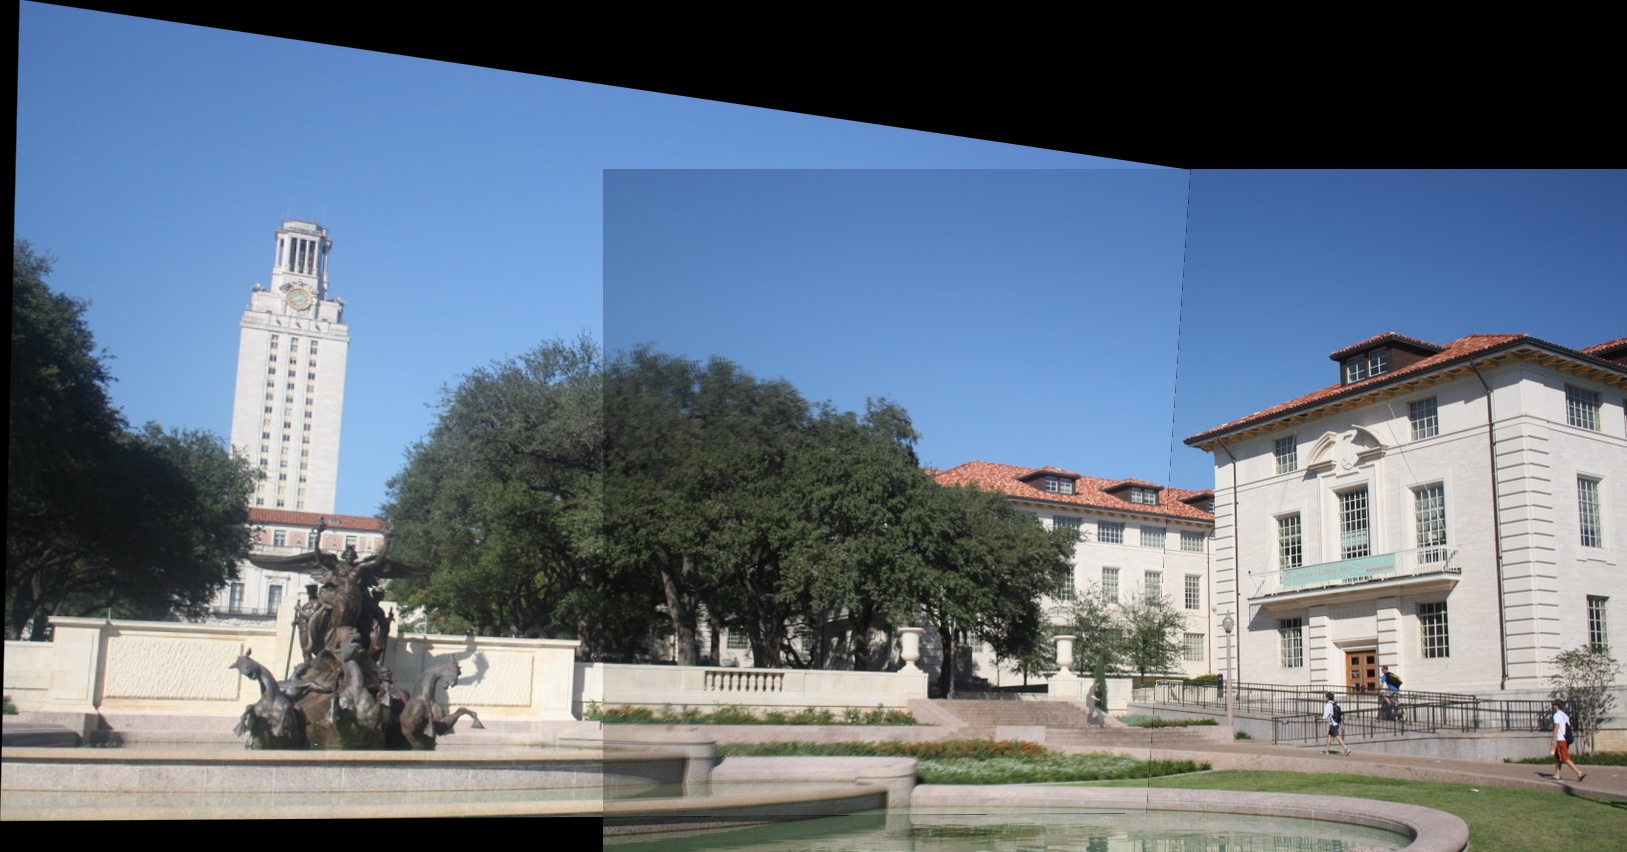
\includegraphics[width=0.7\paperwidth]{pano-tower.jpg}}
\end{center}

{\bf Section 2.2 - Extra Credit:} 

I created panoramas for the extra credit images using the method explained in step 7 of section 1.
The details on the number of inliners for the extra credit images and the transformation matrices used can be found in output/output.txt

Below are the outputed images:
\begin{center}
  \makebox[\textwidth]{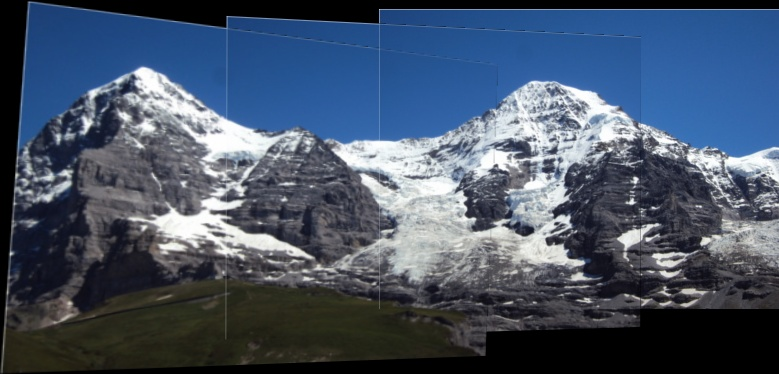
\includegraphics[width=0.7\paperwidth]{pano-hill.jpg}}
  \makebox[\textwidth]{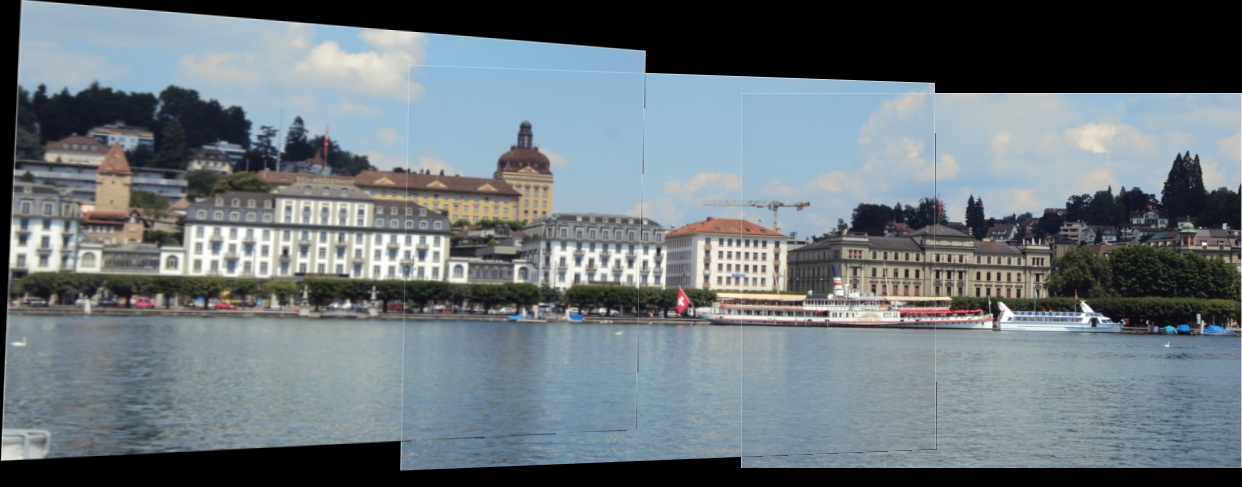
\includegraphics[width=0.7\paperwidth]{pano-pier.jpg}}
  \makebox[\textwidth]{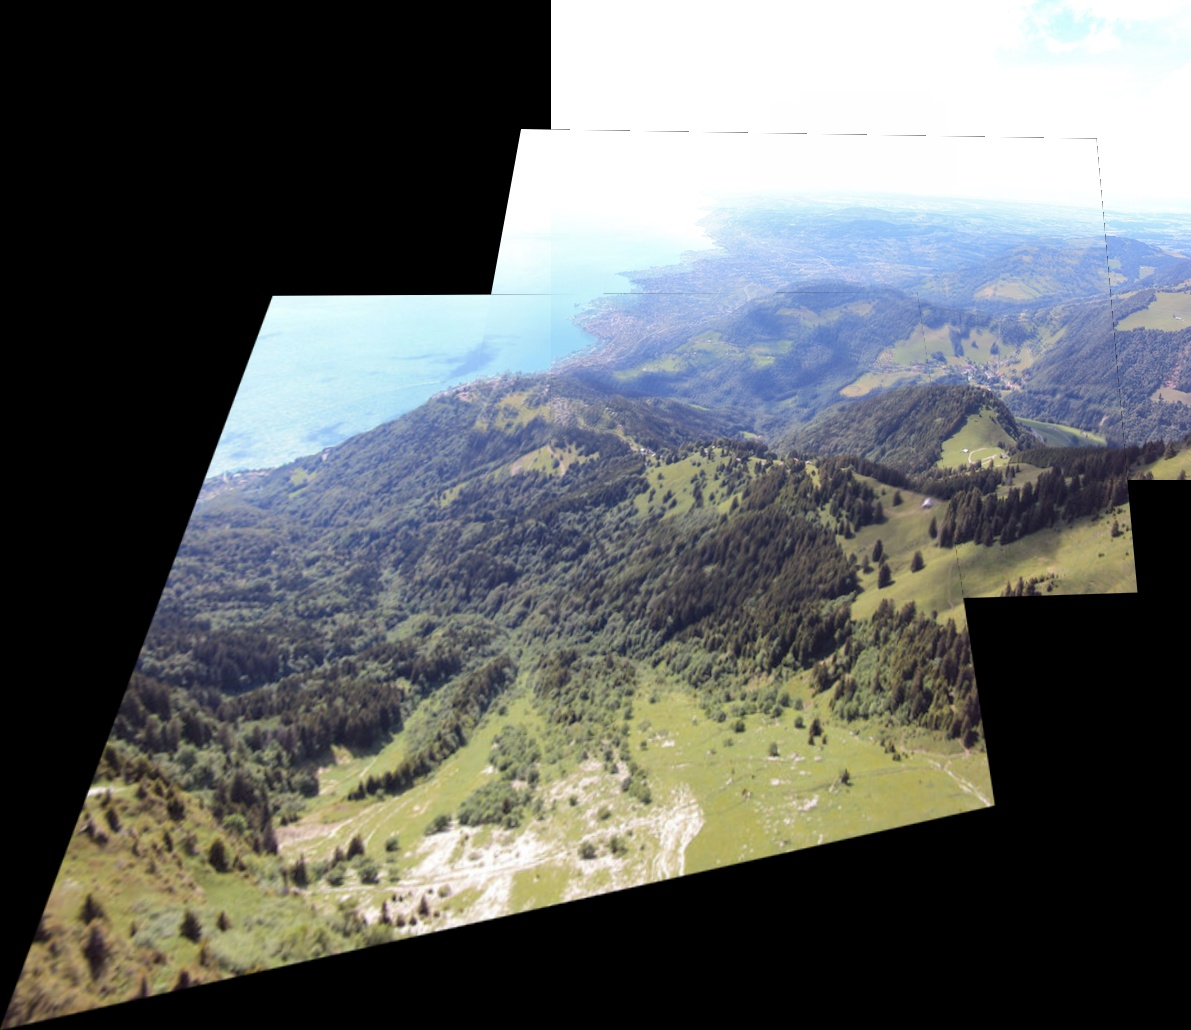
\includegraphics[width=0.7\paperwidth]{pano-ledge.jpg}}
    (My code had the most trouble with the ledge images).
\end{center}



\end{document}
